\section{Task hierarchy}

\paragraph*{Cloning}
The \texttt{fork} system call invokes \texttt{sys\_clone} to create a new copy of the current \texttt{task\_struct} (the process descriptor). 
This new process, or child, is nearly identical to the parent but differs in a few key aspects:
\begin{itemize}
    \item \textit{PID}: the child is assigned a unique Process ID (PID).
    \item \textit{PPID}: the Parent Process ID (PPID) of the child is set to the parent's PID.
    \item Certain resources, such as pending signals, are not inherited by the child.
\end{itemize}

\paragraph*{Copy-on-Write}
Instead of duplicating the entire process address space during cloning, both the parent and child processes share the same memory pages. 
However, when either process attempts to modify the shared data, a copy of the data is created for that process, ensuring that each process has its own unique copy after a write operation.

\subsection{Operating System initialization}
The initialization of an operating system begins with the execution of a function called \texttt{start\_kernel}. 
This function is responsible for performing the essential operations required by the system's architecture to boot the kernel and initialize the core components of the operating environment.

Once the basic elements of the kernel have been set up, the function \texttt{rest\_init} is invoked. 
Its role is to create a new kernel thread, which calls the \texttt{kernel\_init} function. 
This new thread is assigned a PID of 1 and is responsible for initializing all long-term services that are crucial to the system's ongoing operations.

Before proceeding with other tasks, the system calls the architecture-specific function \texttt{cpu\_idle}, associated with PID 0.
This function places the CPU in a low-power, idle state, waiting for other tasks to be scheduled. 
If no tasks are ready to execute, the CPU remains idle to conserve power. 
This idle process continues running for the entire lifespan of the kernel, ensuring that the CPU efficiently manages power when no active work is available.

\paragraph*{System V}
In System V-based systems, initialization follows a structured approach where all files are scanned and organized into predefined run levels. Each run level represents a specific state of the system, controlling which services and processes should be running. 
The \texttt{init} process starts all services associated with the current run level in parallel, only moving to the next run level once the current one has fully initialized. 
The configuration files that define each run level are called \texttt{rc} scripts. 
However, due to the complexity and time-consuming nature of this sequential approach, a more modern system, known as System D, was developed.

\paragraph*{System D}
In System D (also known as systemd), all initialization tasks are run in parallel, significantly speeding up the boot process. 
The core concept in systemd is the unit, which is a plain text file that defines the details of each service or task required during system startup. 
These units describe how and when services should be started, allowing for efficient, concurrent initialization.
\begin{figure}[H]
    \centering
    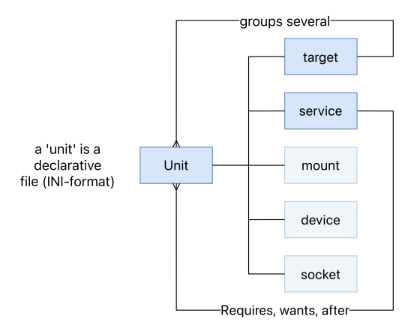
\includegraphics[width=0.75\linewidth]{images/unit.png}
    \caption{System D units}
\end{figure}